% Kompilacja: pdflatex Projekt_ACO_TSP.tex (dwukrotnie).
% Plik samodzielny: nie wymaga zewnętrznych ilustracji ani bibliografii.
\documentclass[11pt,a4paper]{article}
\usepackage[T1]{fontenc}
\usepackage[utf8]{inputenc}
\usepackage{polski}
\usepackage{lmodern,microtype}
\usepackage[margin=2.3cm,top=2.1cm,bottom=2.2cm]{geometry}
\usepackage{amsmath,amssymb,booktabs,tabularx,array}
\usepackage{xcolor,tikz}
\usetikzlibrary{arrows.meta,positioning}
\usepackage{enumitem}
\usepackage[hidelinks,unicode]{hyperref}
\definecolor{ink}{HTML}{243B53}
\hypersetup{pdftitle={Algorytm mrówkowy w problemie komiwojażera},pdfsubject={Opis projektu i plan badań}}
\setlength{\parindent}{0pt}
\setlength{\parskip}{6pt}
\setlength{\emergencystretch}{2em}
\setcounter{tocdepth}{1}
\renewcommand{\arraystretch}{1.25}
\setlist{nosep,leftmargin=1.5em,topsep=4pt}
\newcolumntype{Y}{>{\raggedright\arraybackslash}X}
\newcommand{\plik}[1]{\texttt{\detokenize{#1}}}
\newcommand{\rozdzial}[1]{\clearpage\section{#1}}
\begin{document}

{\small ALGORYTMY INTELIGENTNE INSPIROWANE NATURĄ}
\vspace{1cm}

{\LARGE\bfseries Algorytm mrówkowy\\[5pt]w problemie komiwojażera\par}
\vspace{0.4cm}
{\large Szczegółowy opis projektu i plan badań\par}
\vspace{0.7cm}

\begin{tabular}{@{}ll@{}}
Autorzy & [imię i nazwisko] \\
Grupa & [numer grupy] \\
Prowadzący & [imię i nazwisko] \\
Wersja dokumentu & 1.2 \\
Data & 9 listopada 2026
\end{tabular}

\vspace{0.7cm}
\subsection*{Streszczenie}
Projekt przedstawia zastosowanie algorytmu mrówkowego do wyznaczania krótkiej trasy, która odwiedza wszystkie zadane punkty i wraca do miejsca startu. Problem pokazano na planszy z mrowiskiem i punktami pożywienia. Interaktywna aplikacja pozwala obserwować, jak kolejne iteracje algorytmu wpływają na feromon i najlepszą znalezioną trasę.

Zakres projektu obejmuje implementację algorytmu, wizualizację oraz porównanie z przeglądem zupełnym, najbliższym sąsiadem i metodą 2-opt. Ocenie podlegają długość tras, czas obliczeń i zachowanie po zablokowaniu połączenia. Dokument opisuje istniejącą implementację i sposób jej weryfikacji. Nie przedstawia nowych wyników pomiarów.

\begingroup
\setlength{\parskip}{0pt}
\tableofcontents
\endgroup

\rozdzial{Cel i zakres projektu}
\subsection{Cel projektu}
Celem jest sprawdzenie, czy algorytm mrówkowy potrafi wyznaczać dobre trasy przy rozsądnym koszcie obliczeń. Ważna jest zarówno jakość rozwiązania, jak i możliwość zrozumienia mechanizmu jego powstawania. Z tego powodu część obliczeniową uzupełnia wizualizacja.

Główne pytanie badawcze brzmi: \emph{jak długość tras i czas działania ACO zmieniają się wraz z liczbą punktów oraz jak wypadają na tle innych metod?} Dodatkowo badany będzie wpływ parametrów i przydatność zachowanego feromonu po zmianie kosztu jednej krawędzi.

\subsection{Funkcje programu}
\begin{tabularx}{\textwidth}{@{}p{3.3cm}Y@{}}
\toprule
\textbf{Obszar} & \textbf{Zakres funkcji} \\
\midrule
Edycja planszy & Dodawanie, przesuwanie i usuwanie punktów; przesuwanie mrowiska; losowanie i czyszczenie planszy. \\
Sterowanie & Start, pauza, pojedyncza iteracja, reset feromonu i zmiana parametrów suwakami. \\
Wizualizacja & Rysowanie feromonu, najlepszej trasy oraz historii najlepszej długości. \\
Porównanie metod & Wyznaczenie tras na tej samej planszy i zestawienie ich długości oraz czasu obliczeń. \\
Blokowanie & Zmiana kosztu wskazanego połączenia i obserwacja znalezienia trasy zastępczej. \\
Eksperymenty & Automatyczny zapis tabel CSV i wykresów PNG. \\
\bottomrule
\end{tabularx}

\subsection{Stan realizacji}
Kod zawiera algorytm mrówkowy, trzy metody porównawcze, interfejs Pygame oraz skrypt badań. Są to elementy już zaimplementowane. Ich obecność w kodzie nie zastępuje testów: przed oddaniem projektu należy potwierdzić działanie na komputerze używanym do prezentacji i ponownie przeprowadzić pomiary.

\subsection{Warunki ukończenia}
Projekt będzie gotowy po sprawdzeniu poprawności tras, wykonaniu eksperymentów, opisaniu wyników i ograniczeń oraz przygotowaniu pokazu i prezentacji. ACO nie gwarantuje optimum dla każdego zestawu danych. Ocenie podlega jakość osiągana w określonym budżecie obliczeń.

\rozdzial{Model problemu}
\subsection{Problem komiwojażera}
Na planszy znajduje się mrowisko i $n$ punktów pożywienia. Łączna liczba wierzchołków wynosi $N=n+1$. Mrowisko ma indeks $0$, a pozostałe punkty indeksy od $1$ do $n$. Każdy punkt $i$ ma współrzędne $(x_i,y_i)$.

Szukamy zamkniętej trasy, która zaczyna się w mrowisku, odwiedza każdy punkt pożywienia dokładnie raz i wraca do początku. Kosztem zwykłego połączenia jest odległość euklidesowa:
\begin{equation}
d_{ij}=\sqrt{(x_i-x_j)^2+(y_i-y_j)^2}.
\end{equation}
Odległości są symetryczne: $d_{ij}=d_{ji}$. Przecięcie dwóch odcinków na rysunku nie tworzy nowego wierzchołka.

\subsection{Reprezentacja i ocena trasy}
Trasę zapisujemy jako permutację $\pi=(\pi_0,\ldots,\pi_{N-1})$, gdzie $\pi_0=0$. Powrót do mrowiska jest domyślny. Długość wynosi:
\begin{equation}
L(\pi)=\sum_{k=0}^{N-2}d_{\pi_k,\pi_{k+1}}+d_{\pi_{N-1},\pi_0}.
\end{equation}
Zadanie polega na minimalizacji $L(\pi)$. Poprawna trasa zawiera każdy indeks dokładnie raz. Przy ustalonym początku i symetrycznych kosztach liczba tras różnych z dokładnością do kierunku wynosi $n!/2$ dla $n\geq2$. Już dla 10 punktów pożywienia daje to $1\,814\,400$ możliwości, co uzasadnia ograniczenie przeglądu zupełnego do małych instancji.

\subsection{Model blokady}
Zablokowane połączenie otrzymuje w implementacji koszt $10^6$. Jest to kara kosztowa, a nie usunięcie krawędzi. Taki mechanizm zniechęca algorytmy do korzystania z połączenia, ale nie gwarantuje jego pominięcia. Trasa zawierająca blokadę musi więc zostać rozpoznana jako niedopuszczalna przez osobną kontrolę.

W badaniu blokad rozróżniamy długość geometryczną i koszt uwzględniający kary. Jeżeli nie istnieje dopuszczalny cykl, program nie powinien przedstawiać trasy z karą jako poprawnego objazdu. Wartość kary należy interpretować w skali współrzędnych stosowanej w projekcie.

\subsection{Założenia}
Model nie uwzględnia rzeczywistej sieci dróg, ruchu, przepustowości ani czasu obsługi punktów. W badaniach współrzędne są losowane w kwadracie $100\times100$. W aplikacji odległości wynikają z położenia punktów na planszy.

\rozdzial{Algorytm mrówkowy}
\subsection{Zasada działania}
Zastosowano wariant Ant System ze wzmocnieniem najlepszej dotychczas trasy. Sztuczne mrówki budują rozwiązania niezależnie w ramach danej iteracji, korzystając ze wspólnej macierzy feromonu. Dobre trasy otrzymują większe wzmocnienie, a parowanie stopniowo osłabia wcześniejsze ślady.

Feromon jest pamięcią algorytmu. Nie oznacza jednak pewności, że dana krawędź należy do optimum. Losowy wybór punktów umożliwia dalsze poszukiwanie innych rozwiązań.

\subsection{Wybór kolejnego punktu}
Niech $U$ oznacza zbiór nieodwiedzonych punktów, $\tau_{ij}$ ilość feromonu, a $\eta_{ij}=1/d_{ij}$ dla dodatniej odległości. Mrówka znajdująca się w punkcie $i$ wybiera punkt $j\in U$ z prawdopodobieństwem:
\begin{equation}
p_{ij}=\frac{\tau_{ij}^{\alpha}\eta_{ij}^{\beta}}
{\displaystyle\sum_{u\in U}\tau_{iu}^{\alpha}\eta_{iu}^{\beta}}.
\end{equation}
Parametr $\alpha$ określa wpływ feromonu, a $\beta$ wpływ odległości. Kod ustawia widoczność równą zeru dla zerowej odległości. Gdy suma wag jest zerowa, losowany jest jeden z nieodwiedzonych punktów.

\subsection{Aktualizacja feromonu}
Po zbudowaniu tras przez wszystkie $m$ mrówek następuje parowanie i dodanie nowych śladów:
\begin{equation}
\tau_{ij}\leftarrow(1-\rho)\tau_{ij}
+\sum_{k=1}^{m}\Delta\tau_{ij}^{(k)}+e\,\Delta\tau_{ij}^{\mathrm{best}},
\qquad
\Delta\tau_{ij}^{(k)}=
\begin{cases}
Q/L_k,&(i,j)\text{ należy do trasy }k,\\
0,&\text{w przeciwnym przypadku.}
\end{cases}
\end{equation}
Analogiczny depozyt dla najlepszej trasy wynosi $Q/L_{\mathrm{best}}$. Aktualizacja jest symetryczna. Początkowy feromon to $\tau_0=1/(N L_{\mathrm{NN}})$, gdzie $L_{\mathrm{NN}}$ oznacza długość trasy najbliższego sąsiada. Dolna granica $\tau_0\cdot10^{-3}$ zapobiega całkowitemu zanikowi śladów.

\subsection{Przebieg jednej iteracji}
\begin{enumerate}
\item Obliczenie wag wyboru na podstawie feromonu i odległości.
\item Zbudowanie i ocena trasy każdej mrówki, z uwzględnieniem powrotu.
\item Aktualizacja najlepszego znalezionego rozwiązania.
\item Parowanie, depozyty wszystkich mrówek i wzmocnienie elitarne.
\item Zastosowanie dolnej granicy feromonu i zapis wyniku w historii.
\end{enumerate}

\rozdzial{Parametry i metody porównawcze}
\subsection{Ustawienia algorytmu}
\begin{tabularx}{\textwidth}{@{}p{2cm}p{2cm}Y@{}}
\toprule
\textbf{Parametr} & \textbf{Domyślnie} & \textbf{Znaczenie} \\
\midrule
$m$ & 20 & Liczba mrówek budujących trasy w iteracji. \\
$\alpha$ & 1,0 & Siła wpływu feromonu. \\
$\beta$ & 3,0 & Siła preferencji krótkich połączeń. \\
$\rho$ & 0,3 & Część feromonu usuwana podczas parowania. \\
$Q$ & 1,0 & Skala odkładanego feromonu. \\
$e$ & 1,0 & Waga dodatkowego wzmocnienia najlepszej trasy. \\
$T$ & 100 & Liczba iteracji ACO w porównaniu metod. \\
\bottomrule
\end{tabularx}

Zwiększenie liczby mrówek lub iteracji zwiększa budżet poszukiwania, a także czas obliczeń. Duże $\alpha$ może sprzyjać szybkiemu skupieniu kolonii na dotychczasowych trasach. Duże $\beta$ wzmacnia preferencję pobliskich punktów. Wpływ tych zmian wymaga pomiaru; nie należy zakładać, że większa wartość zawsze daje lepszy wynik.

\subsection{Przegląd zupełny}
Metoda sprawdza permutacje punktów i wybiera najlepszą. Pomija trasy odwrócone oraz przerywa ocenę kandydata, gdy częściowy koszt przekracza najlepszy dotąd wynik. Pozostaje metodą o koszcie silniowym. W aplikacji stosowana jest do 10 punktów pożywienia i stanowi dokładny punkt odniesienia dla przyjętej macierzy kosztów.

\subsection{Najbliższy sąsiad}
Od mrowiska przechodzi się do najbliższego nieodwiedzonego punktu, aż odwiedzone zostaną wszystkie. Metoda jest prosta i szybka, lecz decyzje lokalne mogą prowadzić do długich połączeń pod koniec trasy. Koszt działania wynosi $O(N^2)$.

\subsection{Metoda 2-opt}
Metoda rozpoczyna od trasy najbliższego sąsiada. Sprawdza, czy zastąpienie dwóch krawędzi inną parą połączeń i odwrócenie fragmentu trasy skraca rozwiązanie. Zamiany są powtarzane, dopóki występuje poprawa. Wynik jest lokalnie optymalny względem rozważanych zamian, bez gwarancji optimum globalnego. Pełny przegląd par kosztuje $O(N^2)$; liczba przeglądów zależy od danych.

\subsection{Koszt ACO}
Budowanie tras w obecnej implementacji ma koszt rzędu $O(TmN^2)$. Macierze odległości, feromonu i wag zajmują pamięć rzędu $O(N^2)$. W jednej iteracji przechowywane są także trasy mrówek, o rozmiarze $O(mN)$, a historia wyników zajmuje $O(T)$.

\rozdzial{Budowa i obsługa programu}
\subsection{Podział odpowiedzialności}
\begin{tabularx}{\textwidth}{@{}p{3.7cm}Y@{}}
\toprule
\textbf{Plik} & \textbf{Odpowiedzialność} \\
\midrule
\plik{algorytmy.py} & Macierz odległości, ocena tras, blokady, cztery metody i klasa \plik{AntColony}. \\
\plik{aplikacja.py} & Interfejs Pygame, edycja planszy, sterowanie i wizualizacja. \\
\plik{porownanie.py} & Serie eksperymentów, agregacja wyników, CSV i wykresy. \\
\plik{requirements.txt} & Zależności projektu. \\
\plik{uruchom.bat} & Utworzenie środowiska i uruchomienie w Windows. \\
\bottomrule
\end{tabularx}

\begin{center}
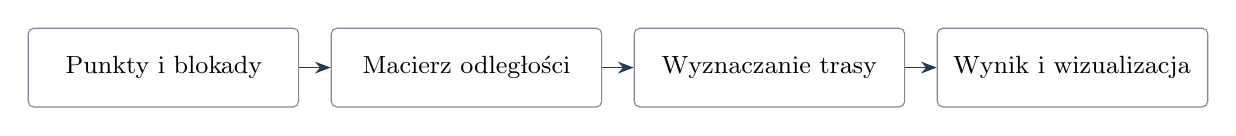
\begin{tikzpicture}[node distance=4mm,every node/.style={font=\small,align=center},box/.style={draw=ink!60,rounded corners=2pt,minimum height=10mm,text width=3.2cm},arr/.style={-{Stealth[length=2mm]},draw=ink}]
\node[box] (a) {Punkty i blokady};
\node[box,right=of a] (b) {Macierz odległości};
\node[box,right=of b] (c) {Wyznaczanie trasy};
\node[box,right=of c] (d) {Wynik i wizualizacja};
\draw[arr] (a)--(b); \draw[arr] (b)--(c); \draw[arr] (c)--(d);
\end{tikzpicture}
\end{center}

Klasa \plik{AntColony} udostępnia \plik{iterate()} do wykonania jednego kroku i \plik{run(iterations)} do serii kroków. Pola \plik{best_tour}, \plik{best_length} i \plik{history} przechowują wynik. Metoda \plik{set_distances} umożliwia zmianę kosztów z zachowaniem feromonu. Zmiana punktów resetuje kolonię. Porównanie w interfejsie uruchamia osobne ACO na 100 iteracji, więc jego wynik może różnić się od aktualnej trasy na planszy.

\subsection{Instalacja i uruchomienie}
Wymagany jest Python 3.10 lub nowszy oraz Pygame, NumPy i Matplotlib. W macOS lub Linux, w głównym katalogu repozytorium, należy wykonać:
\begin{verbatim}
python3 -m venv .venv
source .venv/bin/activate
python -m pip install -r requirements.txt
python aplikacja.py --okno
\end{verbatim}
W Windows można użyć \plik{uruchom.bat}. Eksperymenty uruchamia polecenie \plik{python porownanie.py}; argument \plik{--szybko} zmniejsza część liczby powtórzeń.

\subsection{Sterowanie i pokaz}
Lewy przycisk myszy dodaje i przesuwa punkty, a prawy usuwa punkt pożywienia. Spacja uruchamia lub zatrzymuje ACO, S wykonuje krok, R losuje punkty, a C czyści planszę. B włącza blokowanie, P uruchamia porównanie, F11 zmienia tryb ekranu, a Esc zamyka aplikację.

Pokaz warto rozpocząć od 6--8 punktów: wykonać krok, uruchomić kolonię i porównać wynik z optimum. Następnie zwiększyć liczbę punktów i zablokować krawędź najlepszej trasy. Wpływ parametrów należy pokazywać po resecie feromonu.

\rozdzial{Plan eksperymentów}
\subsection{Zasady porównania}
Wszystkie metody otrzymują te same punkty i tę samą macierz kosztów. Pomiar funkcją \plik{time.perf_counter} obejmuje wyznaczanie trasy, bez generowania instancji, rysowania i zapisu plików. Raport końcowy powinien podawać sprzęt, system, wersje bibliotek, ziarna generatora oraz budżet ACO.

\begin{tabularx}{\textwidth}{@{}p{2.5cm}Y p{4.2cm}@{}}
\toprule
\textbf{Badanie} & \textbf{Ustawienia skryptu} & \textbf{Oceniane wielkości} \\
\midrule
Małe instancje & 3--10 punktów; 5 powtórzeń, w trybie szybkim 2. & Długość względem optimum i czas. \\
Duże instancje & 10, 20, 30, 50, 75 i 100 punktów; 3 powtórzenia, w trybie szybkim 2. & Długość względem najlepszego wyniku metod i czas. \\
Zbieżność & 30 punktów, 150 iteracji, 3 ziarna na każdy z 5 wariantów. & Najlepsza długość po kolejnych iteracjach. \\
Blokada & 20 punktów, 100 iteracji rozgrzewki, do 300 iteracji adaptacji; 10 powtórzeń lub 3. & Pierwszy objazd i osiągnięcie progu jakości. \\
\bottomrule
\end{tabularx}

Warianty zbieżności obejmują ustawienia domyślne, brak wpływu odległości ($\beta=0$), brak wpływu feromonu ($\alpha=0$), wolne parowanie ($\rho=0{,}05$) oraz szybkie parowanie ($\rho=0{,}8$).

\subsection{Miary jakości}
Względną nadwyżkę długości wyrażamy jako:
\begin{equation}
g=100\%\left(\frac{L}{L_{\mathrm{ref}}}-1\right).
\end{equation}
Dla małych instancji $L_{\mathrm{ref}}$ jest optimum z przeglądu zupełnego. Dla dużych jest najlepszym wynikiem spośród badanych metod, a nie potwierdzonym optimum. Krzywa zbieżności pokazuje najlepszy dotąd koszt, który przy stałej macierzy nie powinien rosnąć.

\subsection{Reakcja na blokadę}
Po rozgrzewce blokowana jest losowa krawędź najlepszej trasy. Porównujemy zachowanie feromonu z uruchomieniem nowej kolonii. Próg dobrej jakości wynosi $1{,}03$ długości wyniku 2-opt na zmienionej macierzy. Trzeba sprawdzić dopuszczalność zarówno trasy odniesienia, jak i wyniku ACO.

\subsection{Raportowanie wyników}
Skrypt zapisuje CSV i wykresy w katalogu \plik{wyniki/}. Oprócz średniej warto podać rozrzut i liczbę sukcesów. Obecnie nieosiągnięcie progu jest zapisywane jako limit 300 iteracji; przed analizą należy odróżnić je od sukcesu w ostatniej iteracji. Dodatkowe uruchomienia ACO na tych samych punktach pozwolą oddzielić wpływ losowości algorytmu od różnic między instancjami.

\rozdzial{Weryfikacja i dalsze prace}
\subsection{Sprawdzenie poprawności}
\begin{tabularx}{\textwidth}{@{}p{3.3cm}Y@{}}
\toprule
\textbf{Przypadek} & \textbf{Oczekiwane zachowanie} \\
\midrule
Kwadrat jednostkowy & Optymalna zamknięta trasa ma długość 4. \\
Struktura trasy & Każdy indeks występuje raz; początkiem jest 0, a koszt obejmuje powrót. \\
Małe instancje & Heurystyka nie uzyskuje kosztu niższego od optimum poza tolerancją numeryczną. \\
Poprawa 2-opt & Końcowa trasa nie jest dłuższa od trasy początkowej. \\
Powtarzalność ACO & Przy tych samych danych, parametrach i ziarnie przebieg jest odtwarzalny. \\
Blokady & Funkcja \plik{uses_blocked} rozpoznaje użycie zablokowanej krawędzi. \\
Przypadki brzegowe & Sprawdzenie małej liczby punktów, punktów nakładających się i braku dopuszczalnego cyklu. \\
\bottomrule
\end{tabularx}

\subsection{Ograniczenia implementacji}
Nakładające się punkty mogą prowadzić do zerowego kosztu trasy i dzielenia przez zero. Należy dodać walidację danych i kosztów. Przegląd zupełny działa synchronicznie, przez co przy górnym limicie może czasowo zatrzymać interfejs. Silne skupienie feromonu może ograniczyć różnorodność poszukiwań, dlatego wyniki ACO wymagają wielu uruchomień.

\subsection{Kolejne etapy}
\begin{enumerate}
\item Uruchomić aplikację w docelowym środowisku i wykonać testy kontrolne.
\item Doprecyzować obsługę niedopuszczalnych tras i nieosiągnięcia progu.
\item Przeprowadzić pełne eksperymenty i zachować dane źródłowe pomiarów.
\item Uzupełnić raport o wykresy, interpretację i wnioski oparte na wynikach.
\item Przygotować prezentację i przećwiczyć demonstrację programu.
\end{enumerate}
Terminy etapów należy dopasować do grupy i potwierdzonego harmonogramu trzecich zajęć. Nie przypisano dat zajęć na podstawie samej informacji o ich zamianie.

\subsection{Zakres prezentacji}
Proponowany układ to osiem slajdów: cel projektu, model problemu, zasada ACO, parametry i iteracja, budowa programu, pokaz interfejsu, plan badań lub zweryfikowane wyniki oraz ograniczenia i dalsze prace.

\subsection{Materiały projektu}
Źródła opisu stanowią kod i dokumenty repozytorium: \plik{README.md}, \plik{opis_projektu_ACO_TSP.txt}, \plik{algorytmy.py}, \plik{aplikacja.py}, \plik{porownanie.py} oraz dotychczasowa dokumentacja Word. Repozytorium: \url{https://github.com/mmaj1/Genetyczne}.

\end{document}
